% latex template for a article
% written by Michael McClintock

\RequirePackage[l2tabu, orthodox]{nag} % warnings for obsolete stuff
\documentclass[11pt, a4paper]{article}  % article class

% font setup
\usepackage{ifluatex}
\ifluatex
    \usepackage[no-math]{fontspec} % keep standard math
    \setmainfont[Ligatures=TeX]{Linux Libertine}
    \setsansfont[Ligatures=TeX]{Linux Libertine}
    \setmonofont[Ligatures=TeX]{Inconsolata}
\else
    \usepackage[T1]{fontenc}
    \usepackage{inconsolata}
\fi
\usepackage{microtype}

% useful packages
\usepackage[svgnames]{xcolor}          % color commands
\usepackage{graphicx}                  % including graphics (use eps)
\usepackage{multicol}
\usepackage[margin=15mm]{geometry}     % set margins
\usepackage{amsmath,amssymb,cancel,bm} % math \bm for bold math
\usepackage[hidelinks]{hyperref}       % clickable links
\usepackage{url}                       % format urls
\usepackage{cleveref}                  % convenient refrencing use \Cref
\usepackage{paralist}                  % compact itemize/enumerate
\usepackage[hang, small, bf, margin=20pt]{caption} % captions for figures
\usepackage{setspace}%\onehalfspacing               % 1.5 line spacing
\setlength{\parindent}{0cm}\usepackage{parskip}    % paragraph skip
\usepackage[                                   % SI units
    load-configurations=abbreviations,         % unit abrev.
    separate-uncertainty=true,                 % plus minus in uncertainty
    inter-unit-product=\ensuremath{{}\cdot{}}, % dot between units
    per-mode=symbol-or-fraction                % per style
]{siunitx}
% \usepackage{todonotes} % use \todo{blah blah} options inline/noline/nolist/color
% \usepackage{minted}  % code highlighting requires pygments
% \usepackage[english]{babel} % other languages
% \usepackage[nottoc,numbib]{tocbibind} % refs in toc

\begin{document}

\begin{center}
    \rule[0.5ex]{1\columnwidth}{1pt}
    \\[4mm]
    \textbf{\textsc{\Huge Digital Notebooks for Computation}}
    \\[6mm]
    \textit{\Large IPython Notebooks: A classy interface for scientific
    computing}
    \\[6mm]
    \textsc{\large By Michael McClintock}
    \\[4mm]
    \rule[0.5ex]{1\columnwidth}{1pt}
\end{center}

\begin{multicols}{2}

Some people are really good at solving problems with pen and paper. There is
just something special about solving a problem with nothing more than your
mind, a pen and some paper.

When you're done there is a feeling of value associated with your pages of
notes and derivations. If you write it clearly with comments, well all the
better, because now you can share it with others and there is a good chance
they will be able to follow along. This is all well and good until you want to
do some number crunching. For a wide range of problems a computer based
solution is orders of magnitude more effective.

For some people, once we enter the computational realm things get complex and
unclear. There are command lines, compilers, libraries, dependencies, formats
and many other scary things. Try asking someone working with scientific
computations how they solved their problem. More often than not you will get a
very technical answer to a physical problem. What is worse, try asking them to
\emph{show} you how they solved the problem. They tend to give you some
confusing source code and maybe some graphs. Even solving simple problems can
lead to unwieldy solutions.

Next is the often \emph{steep} learning curve associated with computational
tools. There are some amazing tools out there but sometimes you just don't
feel like learning another gigantic piece of software from scratch when all
you want are some simple computations. Wouldn't it be nice to work using a
medium that is clear, elegant and powerful. An environment where your
computational solution is contained and presentable ``as is'' just like a pen
and paper solution.

Recently there has been a push to create systems where computer based
solutions can be written, executed and presented in a format which looks and
\emph{feels} like the traditional pen and paper approach. Brian Granger, a
Physics Professor at California Polytechnic State University and lead
developer of IPython Notebooks, associates data processing with storytelling.
\cite{granger}

\begin{quote} 
\textit {Data is useless on its own, you need to leverage the data to tell a
story.}
\end{quote}

For scientific computation the story is best told using a mix of comments,
code, equations, interactive visualizations and graphs. Finding the perfect
mix when presenting your work is a challenge. The power of digital notebooks
is to let you do all this at one interface and save the result in one format
so it is easy for people to follow along.

You may be familiar with some systems for creating ``interactive digital
notebooks'' or ``computable documents''. Mathematica provide a very popular
solution which exposes the Mathematica language in a visually pleasing format.
\cite{mm}

\begin{quote}
\textit{ Mathematica notebooks are structured interactive documents that can
contain text, graphics, sound, calculations, typeset expressions, and user
interface elements.}
\end{quote}

The idea may also be familiar to programmers. Literate programming is a
similar approach where source code and formatted text are fused into a more
visually pleasing format that can still be executed on a computer. More
recently a solution called IPython Notebooks has been developed which utilizes
the python programming language. IPython Notebooks are an open-source, web-
based, interactive computing environment. Below is a simple example of a
IPython Notebook.

\begin{center}
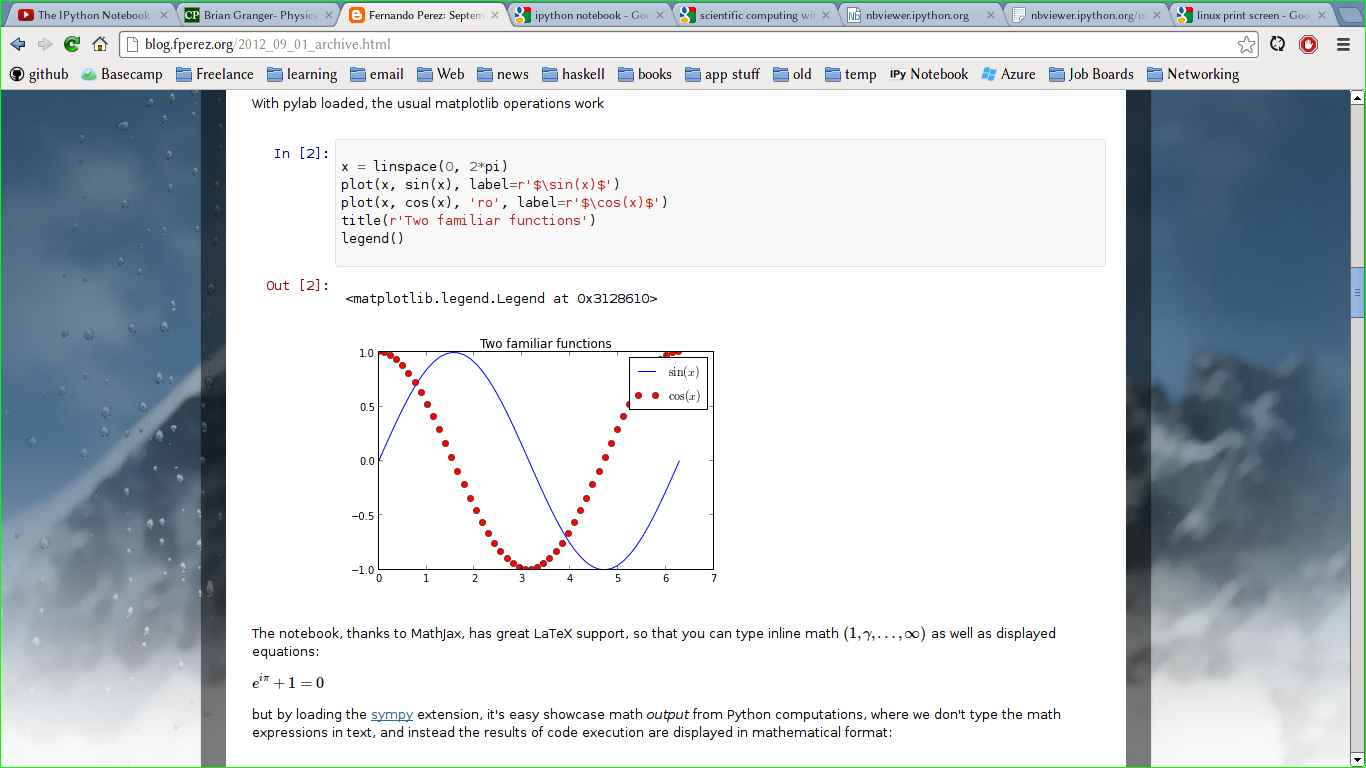
\includegraphics[width=0.45\textwidth]{pic.png}
\end{center}

In case you've been living under a rock, python has become a popular language
for scientific computing. This may be due to its availability (it's free),
clear syntax, ecosystem of high quality libraries and the vibrant python
community. In particular high performance libraries such as Numpy, Scipy and
Matplotlib \cite{py} help create a Matlab-like environment where computational
scientists thrive.

Here are some of the features that IPython notebooks provide.

\begin{itemize}
\item You can write, edit and build everything from right within your browser.
The computations are handled behind the scenes on your computer by
IPython.
\item You can write python code that appears in different blocks in the
notebook. Each block of code can utilize the full power of python and all its
libraries. Its even easy to execute R commands for statistical methods.
\item The cells can be surrounded with areas of formated text (Headings,
paragraphs etc.)
\item Equations can be entered in Tex format which are then typeset when
viewing the notebook
\item Images and videos can be embedded and are often built from some code that
exists at some other point in the notebook.
\item The whole notebook is interactive. Which means any block of text or code
can be edited and re-run where the results show up immediately.
\item To work on your notebooks its as easy as launching IPython and opening
up a browser.
\item Because notebooks are stored in a standard JSON format they can be
easily shared.
\end{itemize}

There are some very nice benefits of uncoupling the user interface (browser)
used to view notebooks from the computational resource (computer running
IPython). It becomes possible, even easy to run your notebooks on high
performance computers or clusters over the web. This opens the door for data
intensive, scalable notebooks that would be inconvenient to run on your laptop
computer. 

These days with services like Amazon EC2 \cite{ec2} and Windows Azure
\cite{azure} it is possible to rent a large number of computing resources.
With these services its rather straightforward to run data intensive IPython
Notebooks ``in the Cloud'' for processing gains. For instance NotebookCloud is
a web-app created for exactly this purpose. This is from NotebookCloud
documentation.

\begin{quote}
\textit{NotebookCloud is service that allows you to launch and control IPython
Notebook servers on Amazon EC2 from your browser. This enables you to host
your own Python programming environment, on your own Amazon virtual machine,
and access it from any modern web browser. You can set everything up in a
minute or two, and it's very easy to use.}
\end{quote}

So its perhaps no surprise that the technology has become increasingly popular.
Fernando Perez the creator of IPython recently wrote. \cite{perez}

\begin{quote}
\textit{Since the notebook was introduced with IPython 0.12, it has proved to
be very popular, and we are seeing great adoption of the tool and the
underlying file format in research and education}
\end{quote}

But rolling code, formated text, equation rendering and multimedia support
into an interactive document isn't something new. As mentioned before
Mathematica Notebooks have been providing scientists and students with elegant
interactive goodness for quite some time. There even exist other more open
notebook systems like Sage Notebooks \cite{sage}. So why all the excitement
about IPython's solution?

Well IPython notebooks are built from ground up using well established open
standards. The format itself is JSON which is used prolifically in software and
web applications for storing and transferring data. Text can be entered in
Markdown which is also hugely popular being the text format of choice for
popular websites such as StackOverflow, Reddit and Github. Equations can be
entered in TeX notation which will most likely be familiar to scientists
everywhere. Even the final result is standards-based. Its just HTML in a
browser.

With all these well established open technologies IPython notebooks have all
the right ingredients to appeal to scientists, IT professionals and students.
In fact educators and lectures have been quick to see the value of IPython
notebooks as learning tools. Dr. C. Titus Brown is a assistant professor at
Michigan State University who has been using IPython notebooks for teaching
classes. Dr. Brown recently wrote about his experience of using IPython in a
classroom environment. \cite{brown}

\begin{quote} 
\textit{The IPython Notebook (or ``ipynb'' for short) is one of the most
exciting technologies for teaching and research that I've seen in recent
years. It is a completely open source, well architectured, and fairly stable
system for scientific computing and data exploration.}
\end{quote}

\begin{quote}
\textit{\textbf{The bottom line is that the IPython Notebook is (still) the
best thing I've ever used for teaching.}}
\end{quote}

It's not just educators and rookie students who find IPython notebook
appealing. As written on his website Randy Olsen is a PhD student at Michigan
State University. Here are his thoughts on the software. \cite{olson}

\begin{quote}
\textit{I do the majority of my post-experiment data analysis in Python
nowadays, since its one of the few sanely-designed scripting languages out
there with all the functionality I need. What I've been missing is a seamless
user interface where I can both take notes about my research and perform my
data analysis in the same location. IPython Notebook finally provides that.}
\end{quote}

When you share and collaborate on a project in a structured environment the
results can be nothing short of amazing. With the growing number of internet
tools and social media outlets it is becoming possible and even essential to
collaborate online. One of the biggest success stories for this approach is
Github.com \cite{gh}. Github is a website where mainly programmers and
software engineers work on opensource projects using the popular version
control system Git. The quality, scale and popularity of the Github ecosystem
is amazing.

Github like systems have been widely accepted in the IT community which have
benefited greatly as a result. However there is nothing specific about these
``Social Coding'' environments that make them unsuitable for scientists and
students. Combining online ecosystems like GitHub with scientific computing
tools like IPython Notebooks may provide a \emph{potent} mix where students,
educators and scientists can collaborate. 

The future looks promising for online learning and collaboration in science.
It is already possible to find examples where students are writing assignments
as IPython Notebooks and managing them on Github. When the due date arrives
the lecturer can mark the notebooks online directly from Github. \cite{brown2}

Only time will tell if the scientific community embraces online collaboration
with tools like IPython Notebook. But is safe to say that this area of
education is rapidly improving. With the astonishing growth of networked
devices like smartphones and tablets along with the ``Cloud Computing''
revolution it seems systems like IPython Notebook will only become more popular
with students and scientists.

\end{multicols}

\bibliographystyle{ieeetr}
\bibliography{refs}

\end{document}
